\documentclass[a4paper,12pt]{article}

% Codificación y lenguaje
\usepackage[utf8]{inputenc}
\usepackage[T1]{fontenc}
\usepackage[spanish]{babel}
\usepackage[utf8]{inputenc}

% Paquetes esenciales
\usepackage{graphicx}
\usepackage{geometry}
\usepackage{datetime}
\usepackage{titlesec}
\usepackage{fancyhdr}
\usepackage{parskip}
\usepackage{array}
\usepackage{float}
\usepackage{placeins}
\usepackage{hyperref}
% Paquetes para código fuente
\usepackage{listings}
\usepackage{xcolor}
\usepackage{amsmath}  

% Configuración del estilo de listings para código Arduino
\lstdefinestyle{arduino}{
  language=C++,
  basicstyle=\ttfamily\footnotesize,
  keywordstyle=\color{blue},
  commentstyle=\color{gray},
  stringstyle=\color{red},
  numbers=left,
  numberstyle=\tiny,
  stepnumber=1,
  numbersep=5pt,
  backgroundcolor=\color{white},
  frame=single,
  breaklines=true,
  captionpos=b
}
\lstset{style=arduino}

% Márgenes del documento
\geometry{left=3cm, right=2.5cm, top=3cm, bottom=3cm}

\begin{document}


\begin{titlepage}
    \begin{center}
        {\LARGE \textbf{Universidad Nacional de Córdoba}}\\[1.5cm]

        
\includegraphics[scale=0.4]{img/logo2.png}\\[1.5cm]

        {\large Facultad de Ciencias Exactas, Físicas y Naturales}\\

        \rule{\linewidth}{0.5mm}\\[0.4cm]
        {\Large \textbf{Cátedra de Arquitectura de Computadoras}}\\[0.3cm]
        {\LARGE \textbf{Trabajo Práctico 1: ALU}}\\[0.3cm]
        \rule{\linewidth}{0.5mm}\\[1cm]

        \begin{flushleft}
        {\large 
            \textbf{Profesores:} - Martin Pereyra, Santiago Rodriguez\\
            \textbf{Integrantes:}\\
            Pallardó Agustín - 
            \href{mailto:apallardo@mi.unc.edu.ar}{apallardo@mi.unc.edu.ar}\\
            Trachta Agustín - 
            \href{mailto:agutrachta@mi.unc.edu.ar}{agutrachta@mi.unc.edu.ar}\\
        }
        \end{flushleft}

        \vfill

        {\large \today}
    \end{center}
\end{titlepage}
\tableofcontents
\clearpage
\section{Introducción}

La comunicación serie es uno de los mecanismos más utilizados en sistemas digitales para transmitir información de manera simple y eficiente. Dentro de este esquema, el estándar \textbf{UART} (Universal Asynchronous Receiver/Transmitter) constituye una de las soluciones más difundidas debido a su simplicidad de implementación, bajo costo y compatibilidad con una amplia variedad de dispositivos.

En este trabajo se presenta el diseño e implementación de un sistema digital basado en \textbf{UART}, desarrollado en lenguaje \textit{Verilog HDL}. El sistema no solo incluye los bloques clásicos de transmisión y recepción, sino que además incorpora:

\begin{itemize}
    \item \textbf{Un generador de baudios} para sincronizar la comunicación.
    \item \textbf{Memorias FIFO} que permiten desacoplar los datos recibidos y transmitidos.
    \item \textbf{Una Unidad Aritmético-Lógica (ALU)} encargada de procesar los operandos recibidos.
    \item \textbf{Un bloque de interfaz} que organiza los datos provenientes del canal serie para dirigirlos a la ALU y reenviar los resultados.
\end{itemize}

El objetivo principal es demostrar cómo la arquitectura UART puede extenderse más allá de la simple comunicación, integrándose con módulos de procesamiento para construir sistemas digitales completos. En particular, se busca implementar un mecanismo mediante el cual se reciben instrucciones desde un puerto serie, se procesan mediante la ALU y los resultados se reenvían nuevamente al transmisor UART.

El trabajo se organiza de la siguiente manera: primero se describen los módulos fundamentales en orden de ejecución (generador de baudios, receptor, FIFO, transmisor, ALU e interfaz). Posteriormente, se analiza la integración en el módulo \texttt{top}, se presentan las simulaciones y pruebas realizadas, y finalmente se discuten los resultados obtenidos junto con posibles mejoras.

\clearpage
\section{Objetivos}

\subsection{Objetivo general}
Implementar y validar una Unidad Aritmético-Lógica (ALU) en una FPGA Basys 3.

\subsection{Objetivos específicos}
\begin{itemize}
    \item Implementar una ALU parametrizable en Verilog, de modo que el ancho del bus de datos pueda ajustarse según futuras necesidades.
    \item Validar la implementación mediante un banco de pruebas (\textit{testbench}) que genere entradas asignadas y contemple un mecanismo de validación.
    \item Integrar la ALU con los periféricos de la Basys 3 (switches, botones, LEDs y display de 7 segmentos) para verificar el correcto funcionamiento en hardware real.
\end{itemize}

\clearpage
\section{Marco teórico}

\subsection{La ALU en el contexto de un procesador}
La Unidad Aritmético-Lógica (ALU) es el bloque funcional encargado de ejecutar operaciones aritméticas, lógicas y de desplazamiento sobre operandos binarios. En un procesador, la ALU recibe los datos desde el banco de registros y ejecuta la operación seleccionada por la unidad de control. Su salida alimenta de vuelta el banco de registros y/o el camino de datos (bus) para su posterior uso. 
En arquitecturas \textit{RISC}, la ALU suele implementar un conjunto mínimo pero completo de operaciones combinacionales de un ciclo, mientras que operaciones más complejas (multiplicación, división) pueden resolverse por hardware dedicado o microcódigo.

\subsection{Representación de datos: complemento a dos y \texttt{signed/unsigned}}
En hardware digital, los enteros con signo suelen representarse en \textit{complemento a dos}. Para un ancho de palabra $N$, el rango representable es:
\[
[-2^{N-1}, \; 2^{N-1}-1]
\]
En Verilog, declarar un bus como \texttt{signed} hace que las operaciones aritméticas y de desplazamiento aritmético consideren el bit más significativo (MSB) como bit de signo. Para operaciones lógicas (\texttt{\&}, \texttt{|}, \texttt{\^{}}) el signo no afecta el resultado, pero sí es relevante en sumas/restas y corrimientos aritméticos.

\subsection{Operaciones implementadas}
La ALU de este trabajo implementa las siguientes operaciones (las etiquetas son códigos de 6 bits que representan la operación seleccionada por \texttt{i\_op}):

\begin{center}
\begin{tabular}{|c|c|l|}
\hline
\textbf{Código} & \textbf{Operandos} & \textbf{Descripción} \\
\hline
100000 & ADD & Suma de \texttt{i\_data\_a} e \texttt{i\_data\_b} (enteros con signo). \\
100010 & SUB & Resta \texttt{i\_data\_a - i\_data\_b} (con signo). \\
100100 & AND & AND bit a bit. \\
100101 & OR  & OR bit a bit. \\
100110 & XOR & XOR bit a bit. \\
000011 & SRA & Corrimiento a derecha \textbf{aritmético}: preserva el bit de signo. \\
000010 & SRL & Corrimiento a derecha \textbf{lógico}: ingresa ceros por la izquierda. \\
100111 & NOR & NOR bit a bit: \texttt{\textasciitilde (A | B)}. \\
\hline
\end{tabular}
\end{center}

\subsection{Corrimientos: aritmético vs. lógico}
\begin{itemize}
    \item \textbf{SRA} (Arithmetic Right Shift) preserva el bit de signo: si el operando es negativo, se rellenan unos por la izquierda. Esto aproxima una división entre 2 para enteros con signo (redondeo hacia $-\infty$ en representación a dos).
    \item \textbf{SRL} (Logical Right Shift) inserta ceros por la izquierda, apropiado para datos sin signo o para manipulación de campos de bits.
\end{itemize}
Al parametrizar el ancho de dato a $N$ bits, el corrimiento máximo significativo es $N-1$. Es buena práctica enmascarar la magnitud de corrimiento con $\log_2(N)$ bits para evitar comportamientos dependientes de la herramienta:
\[
\texttt{shift\_amt} = \texttt{i\_data\_b[} \lceil\log_2(N)\rceil \texttt{-1:0]}
\]

\subsection{Parametrización por ancho de datos}
La ALU se parametriza mediante \texttt{NB\_DATA} (ancho de datos) y \texttt{NB\_OP} (ancho del código de operación). Esto permite reutilizar el diseño para 8, 16 o más bits cambiando sólo parámetros de síntesis, sin modificar el cuerpo del módulo.

\subsection{Señales de estado (flags) y saturación (consideraciones)}
En esta práctica no se implementan \textit{flags} (Carry, Zero, Overflow, Negative) ni saturación; el resultado aritmético se trunca a \texttt{NB\_DATA} bits (comportamiento de \textit{wrap-around}). En extensiones futuras se pueden agregar:
\begin{itemize}
    \item \textbf{Zero}: \texttt{o\_result == 0}
    \item \textbf{Negative}: \texttt{o\_result[NB\_DATA-1]}
    \item \textbf{Carry/Overflow}: a partir del bit extra en la suma/resta.
    \item \textbf{Saturación}: limitar el resultado al máximo/mínimo representable.
\end{itemize}

\subsection{Multiplexado de display de 7 segmentos}
La Basys 3 posee 4 dígitos de 7 segmentos con \textit{ánodo común}, controlados por líneas \texttt{o\_an} (bajo activo) y segmentos \texttt{o\_seg} (bajo activo). Se multiplexan los dígitos activando uno por vez a alta velocidad. 
En este diseño:
\begin{itemize}
    \item Se usa un contador de 16 bits (\texttt{div}) a 100\,MHz.
    \item La selección \texttt{sel = div[15:14]} genera 4 estados, uno por dígito.
    \item La tasa de avance de estados es $\frac{100\text{ MHz}}{2^{14}} \approx 6103$\,Hz; el refresco por dígito es $\frac{6103}{4} \approx 1526$\,Hz, suficiente para evitar parpadeo.
    \item Se muestra el \textbf{resultado} de la ALU en hexadecimal (2 dígitos activos; los superiores en cero).
\end{itemize}

\clearpage
\section{Desarrollo}

\subsection{Descripción general de la arquitectura}
La arquitectura implementada se compone de cinco bloques principales:
\begin{enumerate}
    \item \textbf{ALU}: bloque combinacional parametrizable que ejecuta las operaciones definidas por \texttt{i\_op}.
    \item \textbf{TOP}: bloque secuencial que registra operandos A/B y el código de operación a partir de los switches y botones de la Basys 3; además enruta resultados a LEDs y display.
    \item \textbf{Hex\_to\_sseg}: decodifica un nibble hexadecimal (0--F) a segmentos (bajo activo).
    \item \textbf{SevenSeg\_hex}: multiplexa cuatro dígitos, selecciona el nibble a mostrar y controla \texttt{o\_an}/\texttt{o\_seg}.
    \item \textbf{Testbench}: banco de prueba autocontenible que aplica estímulos representativos y observa salidas.
\end{enumerate}

\subsection{ALU: consideraciones de diseño}
\paragraph{Interfaz y parámetros.}
La ALU recibe dos operandos \texttt{signed} de \texttt{NB\_DATA} bits y un código de operación de \texttt{NB\_OP} bits. La salida \texttt{o\_result} es \texttt{signed} y del mismo ancho que los operandos.

\paragraph{Ruta de datos interna.}
Se utiliza un registro interno \texttt{r\_result} de \texttt{NB\_DATA+1} bits para computar resultados de suma/resta con un bit extra (posible acarreo/overflow). Finalmente se asigna a \texttt{o\_result} truncando a \texttt{NB\_DATA} bits (sin saturación).

\paragraph{Operaciones de corrimiento.}
\begin{itemize}
    \item \textbf{SRA}: \verb|i_data_a >>> i_data_b|. 
    Al ser \verb|i_data_a| \texttt{signed}, el operador \verb|>>>| replica el bit de signo. 

    \item \textbf{SRL}: se fuerza lógico enmascarando el corrimiento:
    \lstinline|$unsigned(i_data_a) >> i_data_b[$clog2(NB_DATA)-1:0]|.
\end{itemize}

\begin{sloppypar}
\textit{Recomendación de robustez:} también enmascarar el corrimiento en SRA con \texttt{i\_data\_b[\$clog2(NB\_DATA)-1:0]} para hacer explícito el límite del ancho, evitando dependencias de implementación.
\end{sloppypar}

\paragraph{Estilo de codificación.}
El bloque es combinacional (\texttt{always @(*)}) con asignaciones bloqueantes para la lógica interna; las señales de salida se asignan por \texttt{assign}. Este estilo evita \textit{latches} y facilita el mapeo a LUTs/sumadores del FPGA.

\subsection{TOP: captura de entradas y ruteo de salidas}
\paragraph{Captura de operandos y operación.}
\begin{itemize}
    \item \textbf{Reset}: síncrono con \texttt{i\_clk}; limpia registros \texttt{data\_a}, \texttt{data\_b}, \texttt{op}.
    \item \textbf{Botones}: al detectar \texttt{i\_btn\_a}, \texttt{i\_btn\_b}, \texttt{i\_btn\_op} se capturan respectivamente \texttt{i\_sw\_data} (operandos) y \texttt{i\_sw\_data[NB\_OP-1:0]} (operación).
    \item \textbf{Nota}: en hardware real, los botones \textit{rebotan}. Este diseño funcional no incluye \textit{debounce}; para robustez en placa se recomienda añadir sincronización doble y filtro (p.ej., contador temporal).
\end{itemize}

\paragraph{Visualización en LEDs y display.}
\begin{itemize}
    \item \texttt{o\_led\_now} refleja en tiempo real \texttt{i\_sw\_data} (útil para cargar operandos/códigos).
    \item \texttt{o\_led\_res} muestra el resultado de la ALU.
    \item \textbf{Display 7-seg}: \texttt{disp\_val = \{8'h00, alu\_result[7:4], alu\_result[3:0]\}} muestra el resultado en dos dígitos hex; los dos dígitos altos quedan en cero. El punto decimal (\texttt{o\_dp}) permanece apagado.
\end{itemize}

\subsection{Módulos de visualización}
\paragraph{\texttt{hex\_to\_sseg}.}
Tabla de verdad que mapea un nibble (0--F) a segmentos \textbf{bajo activo}. La Basys 3 utiliza ánodos comunes por dígito y cátodos compartidos para segmentos, por eso la codificación de 0 es \texttt{7'b1000000} (todos los segmentos activos menos el punto).

\paragraph{\texttt{sevenseg\_hex}.}
\begin{itemize}
    \item \textbf{Divisor}: contador de 16 bits a 100\,MHz. Con \texttt{sel = div[15:14]} se recorre cada dígito a $\sim$6.1\,kHz y cada dígito se refresca a $\sim$1.5\,kHz (sin parpadeo).
    \item \textbf{Selección de nibble}: según \texttt{sel} se elige el nibble correspondiente de \texttt{i\_value}.
    \item \textbf{Anodos}: \texttt{o\_an} es bajo activo; se activa sólo el dígito seleccionado.
\end{itemize}
\clearpage
\section{Simulación del \textit{testbench}}

Con el fin de validar el correcto funcionamiento de la ALU y su integración con el bloque \texttt{top}, se desarrolló un \textit{testbench} (\texttt{tb\_top\_alu}) autocontenible. Dicho banco de pruebas aplica estímulos representativos sobre las entradas de la unidad y observa las señales de salida relevantes.

\subsection{Descripción del procedimiento}
El \textit{testbench} genera un reloj de 100\,MHz mediante el proceso \texttt{always \#5 clk = \string~clk} y define tareas (\texttt{tasks}) para automatizar la carga de operandos y operación:
\begin{itemize}
    \item \texttt{load\_A(v)}: coloca el valor \texttt{v} en los switches y pulsa \texttt{btn\_a}.
    \item \texttt{load\_B(v)}: coloca \texttt{v} en los switches y pulsa \texttt{btn\_b}.
    \item \texttt{load\_OP(v)}: coloca el código de operación en los switches (6 bits) y pulsa \texttt{btn\_op}.
\end{itemize}

Se probaron las siguientes secuencias:
\begin{enumerate}
    \item Reset inicial.
    \item $A = -5$ (\texttt{0xFB}), $B = 3$.
    \item \textbf{ADD} $\Rightarrow$ \texttt{0xFE} ($-2$).
    \item \textbf{SUB} $\Rightarrow$ \texttt{0xF8} ($-8$).
    \item Cargar $B=1$ para corrimientos:
        \begin{itemize}
            \item \textbf{SRA}($A,1$) $\Rightarrow$ \texttt{0xFD} ($-3$).
            \item \textbf{SRL}($A,1$) $\Rightarrow$ \texttt{0x7D} ($125$).
        \end{itemize}
    \item \textbf{NOR}($A,1$) $\Rightarrow$ \texttt{0x04}.
\end{enumerate}

\subsection{Resultados}
La Figura~\ref{fig:simulacion_tb} muestra la forma de onda obtenida. Puede observarse que las salidas \texttt{led\_res} y \texttt{led\_now} coinciden con los resultados esperados para cada operación.

\begin{figure}[H]
    \centering
    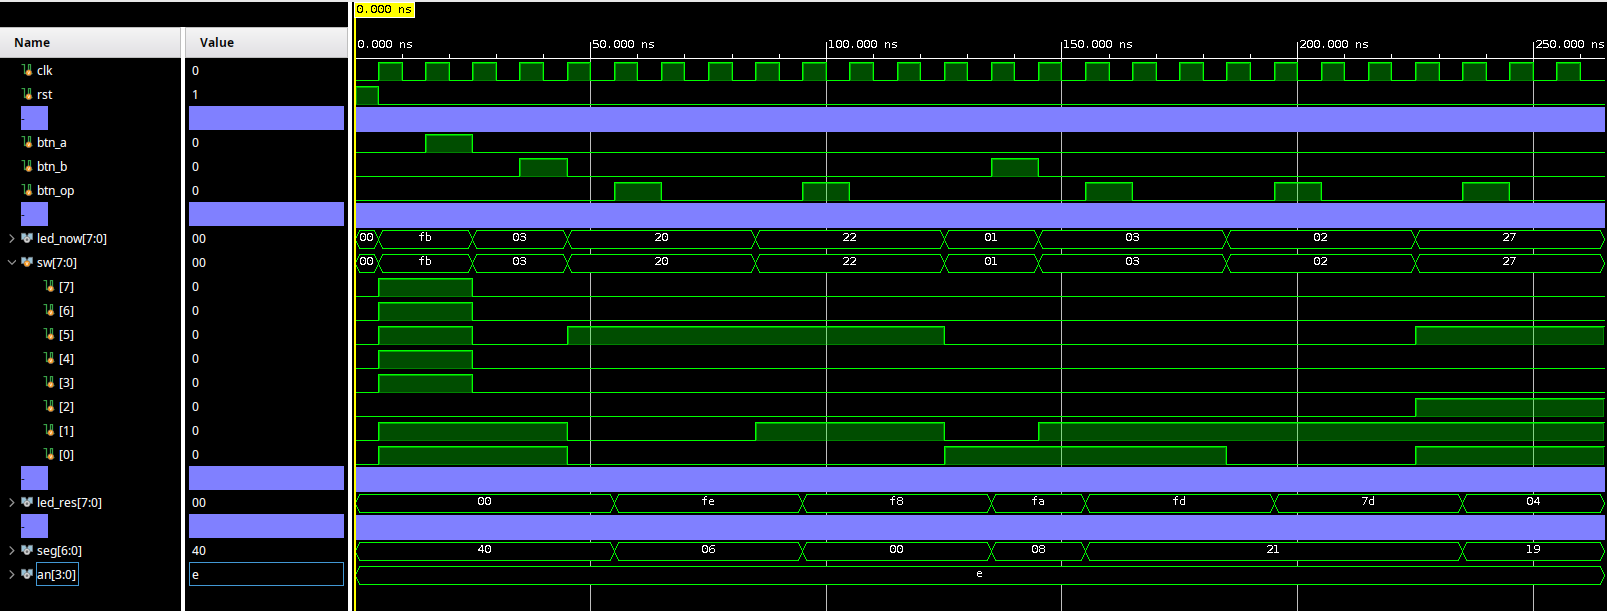
\includegraphics[width=\textwidth]{img/simulacion.png}
    \caption{Forma de onda de la simulación del \textit{testbench}.}
    \label{fig:simulacion_tb}
\end{figure}
\clearpage
\section{Síntesis y diagrama RTL detallado}

A continuación se presentan los diagramas RTL generados por Vivado a partir del código Verilog, que muestran la implementación estructural interna de los módulos principales del diseño.

\subsection{ALU}
En la Figura~\ref{fig:rtl_alu} se observa la implementación detallada de la Unidad Aritmético-Lógica. Cada operación aritmética/lógica se sintetiza en un bloque dedicado (ADD, SUB, AND, OR, XOR, corrimientos aritmético y lógico, INV). Sus salidas se combinan mediante un multiplexor (\texttt{RTL\_MUX}) gobernado por el código de operación \texttt{i\_op}.

\begin{figure}[H]
    \centering
    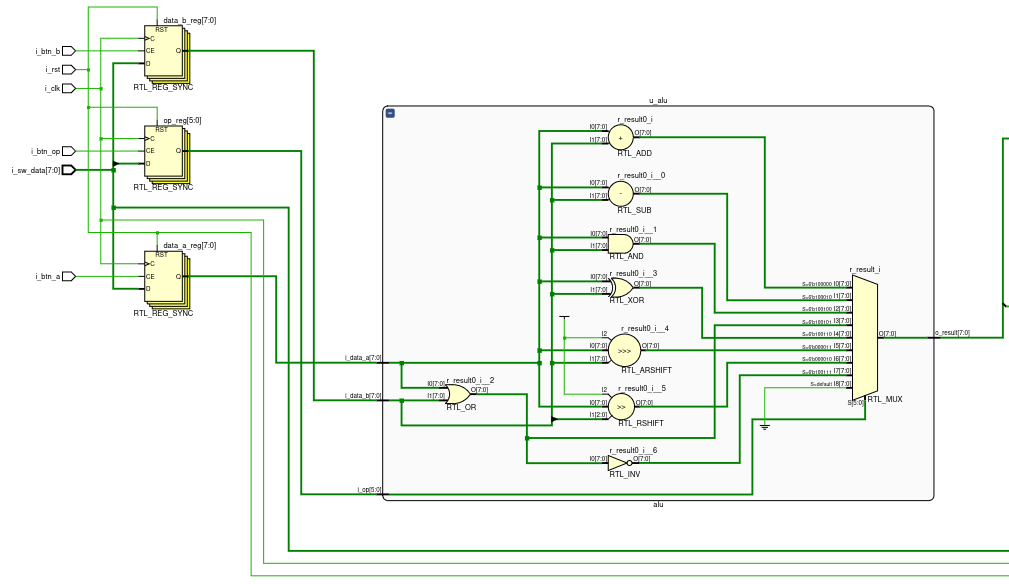
\includegraphics[width=\textwidth]{img/alu.png} % nombre de tu imagen
    \caption{Diagrama RTL del módulo \texttt{alu}.}
    \label{fig:rtl_alu}
\end{figure}

\subsection{Módulo de visualización (\texttt{sevenseg\_hex})}
La Figura~\ref{fig:rtl_disp} muestra el módulo de visualización. El bloque incluye:
\begin{itemize}
    \item Un divisor de frecuencia (\texttt{div\_reg}) que genera la señal de selección de dígito.
    \item Un multiplexor de nibbles (\texttt{RTL\_MUX}) para elegir cuál de los cuatro dígitos se presenta.
    \item Un decodificador hexadecimal a 7 segmentos (\texttt{RTL\_ROM}, \texttt{hex\_to\_sseg}).
    \item Un combinador (\texttt{RTL\_BMERGE}) para activar los ánodos (\texttt{o\_an}) de forma secuencial.
\end{itemize}

\begin{figure}[H]
    \centering
    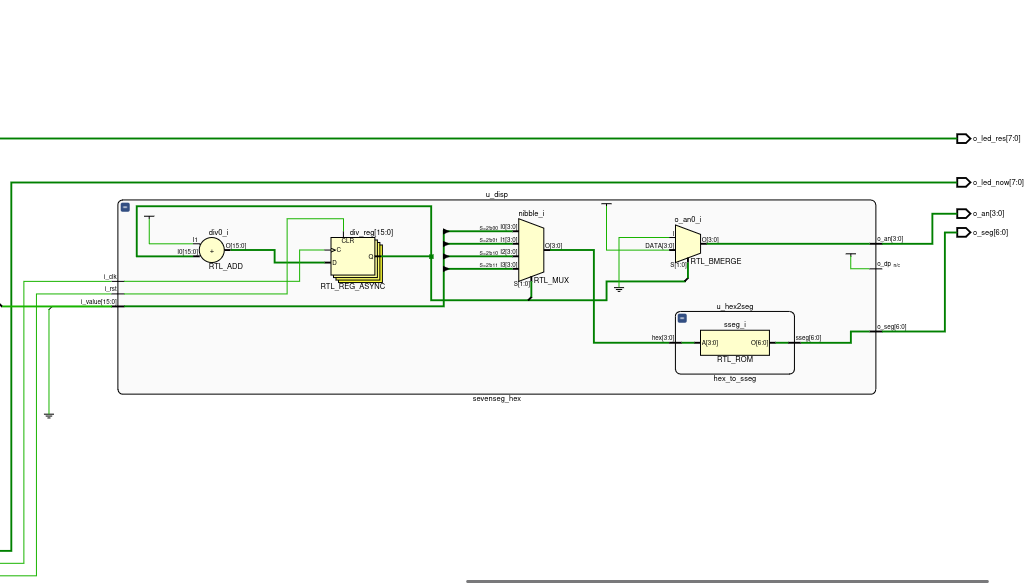
\includegraphics[width=\textwidth]{img/disp.png} % nombre de tu imagen
    \caption{Diagrama RTL del módulo de visualización \texttt{sevenseg\_hex}.}
    \label{fig:rtl_disp}
\end{figure}

\subsection{Módulo \texttt{top}}
Finalmente, en la Figura~\ref{fig:rtl_top} se muestra el diagrama RTL completo del bloque \texttt{top}, que integra los registros de entrada, la ALU y el módulo de display. Se observa cómo las señales de los botones y switches son capturadas en registros sincronizados, las operaciones se ejecutan en la ALU y el resultado se envía tanto a los LEDs (\texttt{o\_led\_res}) como al display de 7 segmentos.

\begin{figure}[H]
    \centering
    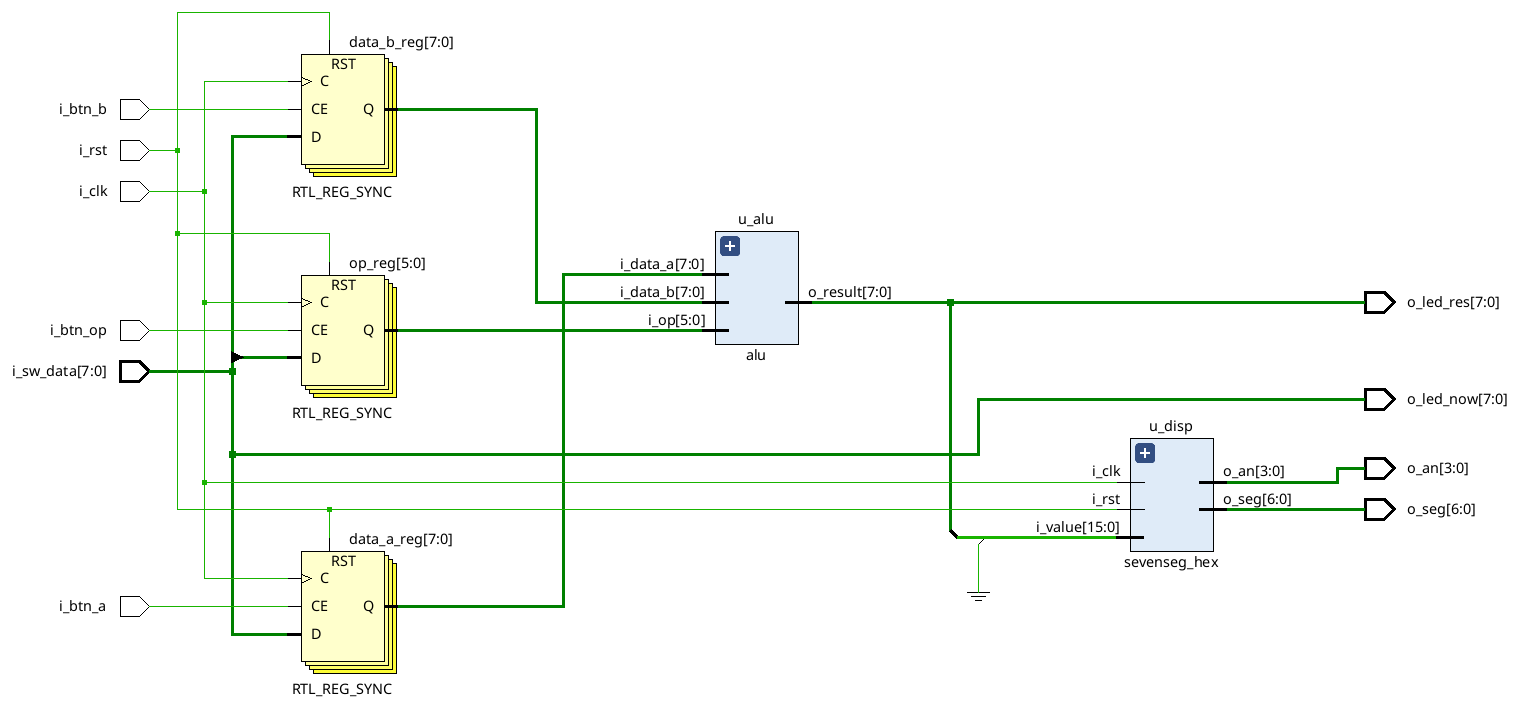
\includegraphics[width=\textwidth]{img/top.png} % nombre de tu imagen
    \caption{Diagrama RTL del bloque superior \texttt{top}.}
    \label{fig:rtl_top}
\end{figure}


\end{document}